% R2 — generality. DRAFT (2026-10-11). Every number is from results/summary_r2_*.csv and
% summary_r2_reading.json (python -m src.analyze_r2); pre-registration: PROJECT_STATUS §10e,
% commit 376382a, and Amendment 1 (Qwen2.5-7B on Kaggle), commit b159fe2 — both before any
% R2 output. Figure: paper/figures/r2_dss.pdf (src/figures_r2.py). Needs: booktabs.
% TODO P8: cite Qwen2.5 (Yang et al. 2024) and Phi-3 (Abdin et al. 2024) technical reports;
% sec:textguard is the P6 section, not written yet.

\subsection{Does the vulnerability generalise beyond one model and one prompt?}
\label{sec:r2}

Model~5 is a single 1.5B-parameter LLM queried with a single prompt. We therefore tested five
further early-fusion forecasters on the same test windows, texts and metrics:
a larger model from the same family, Qwen2.5-7B-Instruct (4-bit NF4, the only way it fits a
16\,GB T4); a model from another family, Phi-3.5-mini-instruct (3.8B, fp16); and Model~5 itself
with three alternative prompts. Two are neutral rewordings: the report placed before the
numbers (\emph{c1}) and reworded instructions (\emph{c2}). The third adds one sentence after
the report, ``this report may be inaccurate or deliberately misleading; check it against the
values above and rely on the values where they disagree'' (\emph{skeptical}). This is the
``just tell the model to be careful'' defence. All runs use greedy decoding and Model~5's
parser and off-scale rule, unchanged. Models, pinned revisions, the exact prompt strings, four
Holm families (one per question; $m = 44, 44, 58, 54$) and the decision rules were
pre-registered before any answer existed. Unlike R1, the pre-registration fixes a smallest
effect size of interest: a forecaster is \emph{fooled} only if its DSS is significantly positive
\emph{and} at least $0.05\sigma$ (at most 13\% of a typical one-step change in any domain).
A non-significant DSS counts as \emph{bounded} only if its whole 95\% CI lies below
$0.05\sigma$; otherwise it is \emph{inconclusive}. Accuracy differences need at least 10\% of
the comparator's MSE, and Flip Rate differences at least 5 percentage points.

\begin{table}[t]
\centering\small
\caption{R2 forecasters on the flip attack (test, pooled over four domains). DSS and Flip
Rate on attacked windows ($n = 246$--$250$); MSE over the 326 test windows with the
available report (each model's valid answers, $n \ge 322$). Verdicts apply the pre-registered rules (Holm within each question's family). Model~5
is from the main experiments and is shown for reference only.}
\label{tab:r2}
\begin{tabular}{lcccl}
\toprule
Forecaster & MSE & DSS (flipped) [95\% CI] & Flip Rate & Verdict (flipped) \\
\midrule
Model~5 (Qwen2.5-1.5B) & 1.055 & $+0.457$ [$+0.348$, $+0.572$] & 23.6\% & (reference) \\
\quad + report first (c1) & 1.083 & $+0.452$ [$+0.319$, $+0.618$] & 28.5\% & fooled \\
\quad + reworded (c2) & 0.862 & $+0.187$ [$+0.121$, $+0.255$] & 12.8\% & fooled \\
\quad + skeptical & 1.303 & $+0.362$ [$+0.260$, $+0.470$] & 20.2\% & fooled \\
Qwen2.5-7B (4-bit) & 0.604 & $+0.206$ [$+0.127$, $+0.293$] & 24.6\% & fooled \\
Phi-3.5-mini & 0.511 & $+0.007$ [$+0.001$, $+0.015$] & 2.4\% & bounded \\
\midrule
Persistence & 0.500 & -- & -- & -- \\
\bottomrule
\end{tabular}
\end{table}

\paragraph{Scale (Qwen2.5-7B).}
The larger model is fooled. It moves $+0.206\sigma$ toward the lie (Holm $p < 10^{-7}$) and
turns 61 forecasts toward the lie against 13 away (Flip Rate 24.6\%). Per domain it is fooled
on Traffic ($+0.247\sigma$) and Health\_US ($+0.323\sigma$), and inconclusive on Economy and
SocialGood. Its manipulation is about half of Model~5's (paired difference $-0.258\sigma$
[$-0.386$, $-0.128$]). The larger model is also more accurate than Model~5 (MSE 0.597 vs 1.061
on the same windows, almost all of the gain on Health\_US). It does not beat persistence:
it is 20\% worse in point estimate, $+0.100$ [$-0.005$, $+0.246$], not significant.
Exaggeration does not push it (bounded, $+0.022\sigma$). So a larger, more accurate LLM is
still steered by a one-word flip. We do not read this as the ``benefits from text and can be
steered'' case our P6 evaluation lacked: removing the report leaves the 7B model's error
unchanged (usage gap $-0.021$ [$-0.182$, $+0.125$]). The effect size also varies across
periods: on the earlier validation split the same model moves only $+0.045\sigma$
[$+0.017$, $+0.073$] toward the lie (Model~5: $+0.270\sigma$). We claim no explanation for
the difference and read the test estimate as one period's value, not a stable constant.

\paragraph{Family (Phi-3.5-mini).}
Phi-3.5's DSS is \emph{bounded} below the SESOI, pooled and in three domains (Traffic
inconclusive), with 6 forecasts turned toward the lie and 1 away. It is bounded because it
ignores what the report says. Its error is within 10\% of
persistence, and lower than Model~5's. An exploratory observation (not pre-registered) shows
why. Without a report Phi-3.5 almost never repeats the last value (1\% of windows). Given
\emph{any} report, real or flipped, it repeats the last value in 73\% of windows (95--97\% on
Health\_US). The report moves its forecast (screening rejects in all four domains), but toward
a flat persistence forecast whatever the report says. A low DSS here measures indifference to
the report's direction, not resistance to misleading text.

\paragraph{Prompt wording.}
Model~5's three P5 conclusions all hold under both rewordings. Both variants are fooled by the
flip (pooled), neither is fooled by exaggeration, and both are moved by text in every domain.
The per-domain pattern agrees with Model~5's in 3 of 4 domains for each. In both cases the
disagreement is SocialGood: inconclusive for c1, bounded for c2, where Model~5 was fooled.
The magnitude depends on the wording. Moving the report first leaves the effect unchanged
($-0.008\sigma$ vs Model~5, n.s.), whereas the reworded instructions reduce it to 41\% of
Model~5's ($-0.283\sigma$, Holm $p = 10^{-4}$). The vulnerability is therefore a property of
the model reading the report, not of one phrasing, but its size is prompt-sensitive.

\paragraph{Telling the model to be careful.}
The skeptical sentence does not remove the manipulation. Model~5 with the caution is still
fooled ($+0.362\sigma$, 50 flips toward the lie vs 3 away). Its reduction against the plain
prompt ($-0.107\sigma$ [$-0.178$, $-0.043$], raw $p = 0.008$) does not survive Holm correction
in the pre-registered family. This gives the pre-registered reading \emph{``prompting does not
help''}. TextGuard v1 at its frozen P6 settings leaves Model~5 at $-0.041\sigma$ on the same
windows, $0.402\sigma$ below the skeptical prompt (Holm $p < 10^{-6}$). Flip rates do not
differ detectably (Table~\ref{tab:r2-sk}). The caution also makes the model react \emph{more}
to genuine reports (text sensitivity $0.461\sigma$ vs $0.388\sigma$). It raises real-text error
on Health\_US ($+0.64$, Holm $p = 0.010$), not significant pooled.

\begin{table}[t]
\centering\small
\caption{Skeptical prompt vs undefended Model~5 and vs TextGuard v1 (frozen P6 settings) on
Model~5 (test, pooled). Differences are skeptical $-$ comparator, paired per window;
Holm within the 54-test R2-d family.}
\label{tab:r2-sk}
\begin{tabular}{llccc}
\toprule
Quantity & Comparator & Difference [95\% CI] & Holm $p$ & Verdict \\
\midrule
DSS & Model~5 & $-0.107$ [$-0.178$, $-0.043$] & 0.30 & no difference detected \\
DSS & TextGuard v1 & $+0.402$ [$+0.283$, $+0.528$] & $1.2\times10^{-7}$ & TextGuard lower \\
Flip Rate & Model~5 & $-3.7$ pp [$-8.2$, $+1.2$] & 1 & no difference detected \\
Flip Rate & TextGuard v1 & $+2.0$ pp [$-3.2$, $+7.3$] & 1 & no difference detected \\
Real-text MSE & Model~5 & $+0.274$ [$+0.098$, $+0.479$] & 0.56 & no difference detected \\
Real-text MSE & TextGuard v1 & $+0.253$ [$+0.005$, $+0.502$] & 0.94 & no difference detected \\
\bottomrule
\end{tabular}
\end{table}

\paragraph{TextGuard v1 on the new models.}
Applied unchanged (its gate depends only on the report and the numbers, so its False Block
Rate stays 14.4\%), TextGuard lowers the 7B model's DSS from $+0.200$ to $+0.087\sigma$
($-0.112$ [$-0.183$, $-0.044$]). The reduction exceeds the SESOI but does not survive Holm
correction (raw $p = 0.014$, Holm $p = 0.36$), so the pre-registered verdict is ``no difference
detected''. On Phi-3.5 there is little to remove ($+0.007 \to -0.015\sigma$, n.s.). There
TextGuard raises the Flip Rate from 2.4\% to 20.4\% while DSS turns slightly negative. This
is an artefact of the Flip Rate definition, not TextGuard following the lie. Phi-3.5's
real-text forecast sits exactly at the last value, and TextGuard pulls the fake-text forecast
off that flat answer toward the model's no-report extrapolation. Our Flip Rate counts any move
from a flat forecast in the claimed direction as a flip, so a forecaster that copies the last
value turns small shifts into flips. We list this as a limitation of the flip definition.

\paragraph{Checks.}
No model shows signs of memorising the test values. No model reproduced a single Economy,
Traffic or Health\_US target exactly. On SocialGood (one-decimal values) at most 4 unexplained
exact matches occur per model and condition, each within 5 percentage points of a placebo rate
computed against the following period (largest excess 4.3 points). Format failures are rare (on test, at most 1.2\% of answers in any model
and condition). They are mostly unit slips on Traffic, plus 8 refusals by Phi-3.5 (2 on test). They are not
concentrated in the fake conditions relative to the real reports the fakes were edited from
(e.g.\ Qwen2.5-7B 0.8\% vs 0.6\%). We chose this yardstick after a first look, and it matches
the comparison of our main experiments. Against all five non-fake conditions pooled, the fake
conditions fail 2--3$\times$ as often, but three of those conditions (no report, a shuffled
report, another domain's report) can hardly produce the dominant failure, a figure copied in the
report's units of billions. Both comparisons are in the released table. Two of 2,282 test answers (Phi-3.5) contain more than one number, and both lead
with the intended forecast.

\paragraph{Reading across R1 and R2 (exploratory).}
Taken together with Section~\ref{sec:r1}, the forecasters split by whether they register a
report's direction. Those that were not fooled ignore it: the BERT heads (whose embedding barely
changes under a flip), the mean-pooled Qwen heads (equally direction-blind; R1's rule counted one
of them fooled at a negligible $+0.0075\sigma$) and Phi-3.5 (which copies the last value
whatever the report says). Those that read the report's direction were steered by it:
Model~5 under all four prompts, Qwen2.5-7B, and the FinBERT heads. The FinBERT heads were
fooled by R1's rule, with effects of $+0.049\sigma$ and $+0.034\sigma$ that fall just below R2's
$0.05\sigma$ SESOI. In our experiments, we found no forecaster that both reads report direction
and resists the attack. This is an observation about 13 forecaster configurations (six model types) on
four domains, not a general law, but it is the use-versus-vulnerability trade-off that motivates an external
check such as TextGuard.

\paragraph{Caveats.}
The 7B model is 4-bit quantised and ran on a different platform (Kaggle) and software stack
from the Colab runs. Its claims are about the quantised model, and its comparisons with
Model~5 are between models. Phi-3.5's bounded DSS comes from ignoring the report's content,
a copying behaviour that also caps its usefulness as a forecaster. The Flip Rate overstates
flips for forecasters that copy the last value (see above). The skeptical sentence is one wording; a stronger instruction could
behave differently.

\begin{figure}[t]
\centering
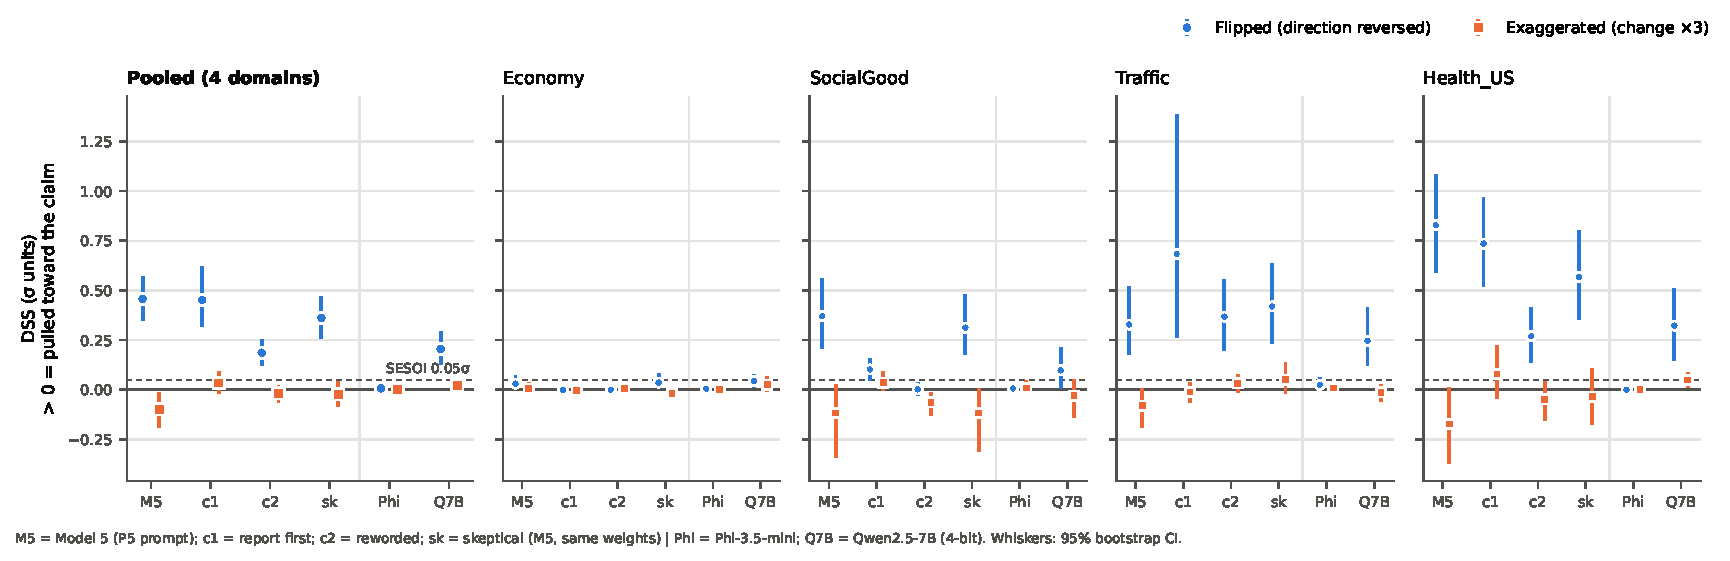
\includegraphics[width=\linewidth]{figures/r2_dss.pdf}
\caption{DSS under the flip (blue) and exaggeration (orange) attacks for Model~5 (M5), its
report-first (c1), reworded (c2) and skeptical (sk) prompts, Phi-3.5-mini (Phi) and
Qwen2.5-7B, 4-bit (Q7B); pooled and per domain, 95\% bootstrap CIs. Dashed: the pre-registered
SESOI ($0.05\sigma$).}
\label{fig:r2-dss}
\end{figure}
